\documentclass[runningheads]{llncs}

\usepackage[T1]{fontenc}
\usepackage{graphicx}
\usepackage{booktabs}
\usepackage{xcolor}
\usepackage{tikz}
\usetikzlibrary{shapes.geometric, arrows.meta, positioning, fit, backgrounds}
\usepackage{url}
\usepackage[hidelinks]{hyperref}

\begin{document}

\title{Concurrent Multi-Platform Social Media Extraction and LLM Sentiment Analysis: A Museum Design Case Study}

\author{Justin Lucero \and Jhonatan Tacuri \and Wilmer Merch\'an}

\institute{Universidad Polit\'ecnica Salesiana, Cuenca, Ecuador \\
\email{jlucerov1@est.ups.edu.ec, jtacuric@est.ups.edu.ec, wmerchang@est.ups.edu.ec}}

\titlerunning{Concurrent Social Media Extraction and LLM Sentiment Analysis}
\authorrunning{J. Lucero et al.}

\maketitle

\begin{abstract}
Social media is a primary channel through which citizens react to public
decisions, but analyzing that reaction at scale is hard: opinions are
scattered across platforms, arrive as unstructured text, and need
context-aware interpretation rather than keyword counting. This paper
presents a web application that extracts, classifies, and interprets social
media opinions concurrently, applying parallel computing and natural
language processing end to end. Given a search query, the system launches
one thread per source and scrapes Facebook and TikTok (Selenium over a
persisted Chrome profile) together with YouTube and Reddit (official REST
APIs), coordinating the platforms that require manual login through a
shared lock so other threads keep working. The consolidated corpus is then
classified by sentiment with a large language model (OpenAI GPT-4o-mini or
Groq Llama-3.1-8b-instant) through a producer--consumer thread pool, and a
rule-based storytelling module turns the statistics into a narrative
interpretation, served through an interactive dashboard. We evaluate the
system on a real case study: public reaction to ``Ecos del Sol'', the
winning design for Ecuador's new National Museum. On a corpus of
508 opinions from three concurrently running sources, classification
processed the full corpus in 49.59\,s and revealed a predominantly negative
sentiment (54.7\%) concentrated on YouTube. A controlled benchmark on an
18-record dataset shows parallel classification reaches a 2.80$\times$
speedup with OpenAI -- near the theoretical maximum for three threads --
while Groq's free tier yields 0.25$\times$ (a slowdown) under concurrent
rate limiting, a limitation often overlooked in I/O-bound parallel designs.
Cross-checking the corpus with both providers yields 83.3\% inter-model
agreement, used as a reliability proxy absent human-labeled ground truth.
These findings show that thread-based concurrency is effective for
I/O-bound social media pipelines, but its benefit is conditioned by the
downstream API's rate-limiting policy, a factor that belongs in the
architectural decision, not as an afterthought.

\keywords{Parallel computing \and Social media mining \and Sentiment
analysis \and Large language models \and Concurrency \and Explainable AI}
\end{abstract}

\section{Introduction}
\label{sec:intro}

Social platforms such as Facebook, TikTok, YouTube, and Reddit have become
one of the largest sources of publicly available opinion data, capturing how
citizens react to political, cultural, and infrastructure decisions in near
real time. This makes them attractive for public-opinion research, but also
hard to analyze: the volume and velocity of new posts outpace manual review,
the text is short, informal, and multilingual, and each platform has its own
access mechanism, data schema, and anti-automation defenses. A system that
wants to answer a question such as \emph{``what do people think about X''}
therefore has to solve three problems at once -- collecting data from several
heterogeneous sources fast enough to be useful, turning unstructured text
into a structured sentiment signal, and presenting the result in a way a
non-technical reader can interpret -- without any of the three becoming the
bottleneck.

This work uses as its case study the public reaction to \emph{``Ecos del
Sol''}, the winning design of an international architecture competition for
Ecuador's new National Museum, which received substantial criticism and
support across social media after being announced. The research question we
address is: \emph{how can a parallel-computing-based system extract, process,
and analyze large volumes of social media data, classifying sentiment and
producing interpretable results efficiently, while applying core computer
science and software engineering principles to the design?}

We propose and implement a web application that answers a user-provided
search query end to end. On submission, the backend launches a thread per
social platform (Facebook, TikTok, YouTube, and Reddit) so that extraction
overlaps rather than executes sequentially; Facebook and TikTok are scraped
through Selenium over a real, persisted Chrome profile, while YouTube and
Reddit are queried through their official REST APIs. The consolidated,
de-duplicated corpus is then classified by sentiment with a large language
model (LLM) using a second, independent thread pool built around a
producer--consumer queue, one worker per source. A lightweight, rule-based
storytelling module turns the resulting aggregate statistics into a
qualitative narrative (dominant sentiment, cross-platform contrast,
engagement-weighted signal, and textual evidence), and all of this is
exposed through an interactive dashboard that lets a user explore individual
opinions together with the LLM's justification for each label.

The main contributions of this paper are: (1) a concurrent, multi-source
social media extraction pipeline that unifies browser-automation and
official-API sources under a single thread-based architecture with shared
login coordination; (2) a parallel, fault-tolerant sentiment classification
stage using a producer--consumer pattern, benchmarked against its sequential
counterpart; (3) an automatic storytelling component that converts aggregate
sentiment statistics into a human-readable interpretation; and (4) an
empirical evaluation on a real 508-opinion corpus that quantifies both the
benefit and a concrete limitation of thread-based parallelism when the
downstream LLM API enforces rate limits.

The rest of this paper is organized as follows. Section~\ref{sec:related}
reviews recent related work on LLM-based sentiment analysis, explainability,
and parallel/distributed processing of social media data. Section
\ref{sec:methodology} describes the system architecture, the concurrency
strategy used at each stage, and the technical decisions behind them.
Section~\ref{sec:results} reports the classification accuracy proxy, the
case-study results, and the execution-time measurements, including the
speedup benchmark. Section~\ref{sec:conclusions} summarizes the main
findings and outlines recommendations for future work.

\section{Related Work}
\label{sec:related}

Table~\ref{tab:related} summarizes six recent works (2023--2025) relevant to
the two axes of this paper -- LLM-based sentiment analysis and parallel
processing of social/textual data -- and positions our system with respect
to each of them.

\begin{table}[p]
\centering
\caption{Recent related work (2023--2025) and its relation to this paper.}
\label{tab:related}
\small
\setlength{\tabcolsep}{4pt}
\renewcommand{\arraystretch}{0.88}
\begin{tabular}{p{2.5cm}p{5.1cm}p{4.1cm}}
\toprule
\textbf{Work} & \textbf{Problem / Method} & \textbf{Relation to our system} \\
\midrule
Kim and Kim \cite{kim2025llm} &
Measures how closely GPT-3.5/GPT-4 Turbo reproduce human-expert sentiment
labels on 1{,}000 Facebook/Twitter posts (few-shot prompting). &
Validates our core design choice of using an LLM (GPT-4o-mini,
Llama-3.1-8b-instant) instead of a human-coded gold set; motivates our
inter-model agreement analysis (Section~\ref{sec:results}) as a reliability
proxy. \\
Sun et al.\ \cite{sun2023sentiment} &
Proposes a two-LLM negotiation (generator/discriminator) framework to reduce
single-pass sentiment errors on ambiguous text. &
An alternative to our single-pass classification step; a natural extension
for future work when higher reliability outweighs latency and cost. \\
Herrera-Poyatos et al.\ \cite{herrerapoyatos2025uncertainty} &
Surveys the ``model variability problem'' in LLM-based sentiment analysis
and argues explainability is necessary for trustworthy deployment. &
Justifies the explainability feature of our dashboard, which shows the
LLM's textual justification next to every label. \\
Chen et al.\ \cite{chen2025shap} &
Combines aspect-based sentiment analysis with a SHAP-interpretable
classifier on social media reviews of cultural heritage sites. &
Closest domain match (public sentiment toward a heritage/architecture
project); differs in using a single-platform corpus and classical ML with
post-hoc explainability instead of multi-platform LLM classification. \\
Li and Wang \cite{li2025shanghai} &
Mines social media reviews to characterize citizen perception of urban
public spaces in Shanghai. &
Single-city, single-corpus analogue of our approach, generalized here to
four concurrently polled platforms and a national landmark. \\
Dixit et al.\ \cite{dixit2023multiprocessing} &
Uses Python multiprocessing to run classifier hyperparameter sweeps
concurrently, reducing training time. &
A CPU-bound parallelism precedent; complementary to our I/O-bound design,
which parallelizes network-bound LLM API calls with threads rather than
processes (Section~\ref{sec:methodology}). \\
Pehlivan et al.\ \cite{pehlivan2025meo} &
Describes a national-scale, multi-platform media observatory with
per-platform crawlers and a schema-normalization layer. &
The closest architectural analogue at a much larger scale; our system
targets a lighter, single-topic deployment with a producer--consumer
sentiment stage and storytelling layer that the observatory does not
include. \\
\bottomrule
\end{tabular}
\end{table}

Beyond these six, the literature confirms two long-standing points our design
builds on. First, lexicon-based sentiment tools such as VADER
\cite{hutto2014vader} and AFINN \cite{nielsen2011afinn} are fast but
struggle with sarcasm, negation, and domain-specific jargon common in social
media comments about public infrastructure -- one of the reasons we adopt an
LLM-based classifier instead. Second, the transformer architecture
\cite{vaswani2017attention} and the pretraining paradigms it enabled, from
BERT \cite{devlin2019bert} to instruction-tuned model families such as
Llama~3 \cite{grattafiori2024llama3} and GPT-4o \cite{openai2024gpt4o}, are
what make it practical to classify sentiment with a short natural-language
prompt (a technique surveyed by Sahoo et al.\ \cite{sahoo2024promptsurvey})
rather than a hand-labeled training set. Regarding data collection, Brown et
al.\ \cite{brown2024webscraping} discuss the ethical and legal
considerations of web scraping for research, which informed our decision to
scrape only public search results through a user-authenticated session
rather than bypassing platform authentication. Finally, Yang and Liu
\cite{yang2022socialmedia} review how social media data has been used in
urban design and landscape research more broadly, providing additional
context for our architecture-related case study, and Hjelle et al.\
\cite{hjelle2024dashboard} provide experimental evidence that dashboard
visualizations measurably improve analytical decision making, which
motivated the design of our exploration and storytelling dashboard.

\section{Methodology}
\label{sec:methodology}

\subsection{System Architecture}

Figure~\ref{fig:architecture} shows the end-to-end architecture. The user
submits a search query and a set of sources through the web front end; a
FastAPI backend creates a background job and immediately returns a job
identifier, so the HTTP request never blocks on the (potentially
minutes-long) extraction and classification work. The job runs in its own
thread and drives three sequential stages, each of which is internally
parallel: concurrent extraction, parallel sentiment classification, and
storytelling generation. Progress is exposed through a polling endpoint that
the dashboard consults every two seconds, including a login checkpoint that
the two Selenium-based sources may need the first time they run.

\begin{figure}[t]
\centering
\resizebox{\textwidth}{!}{%
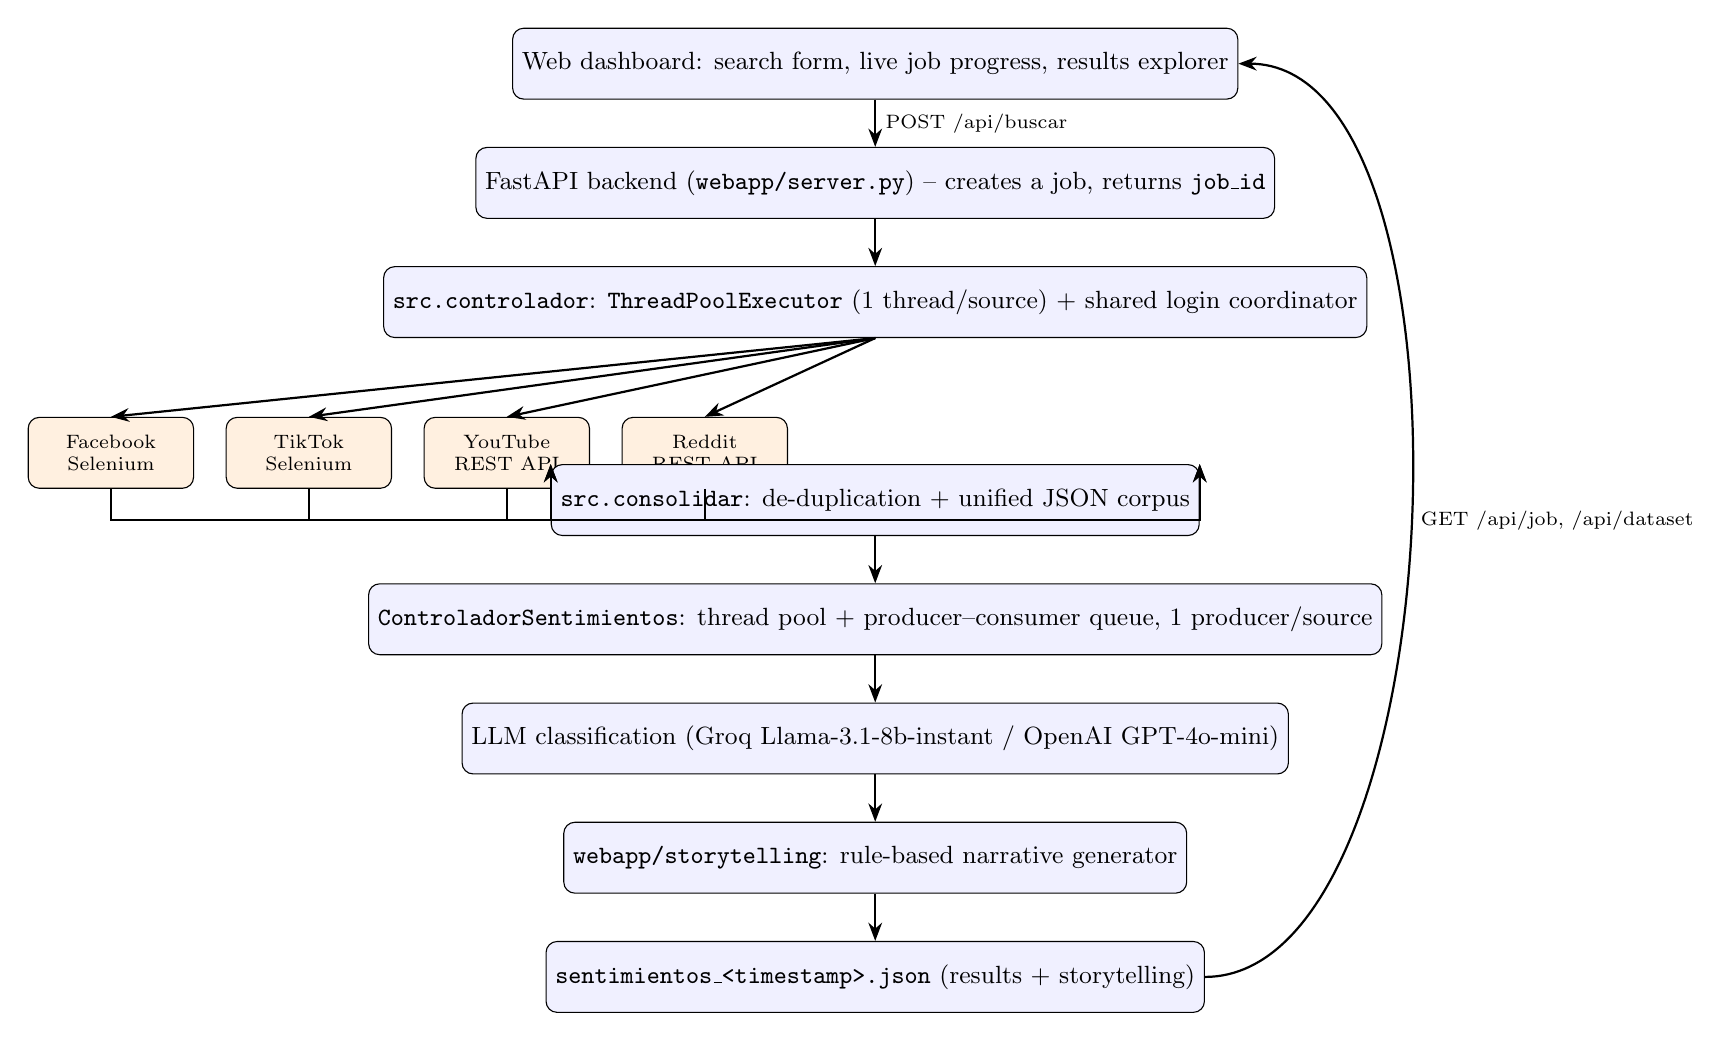
\begin{tikzpicture}[
  node distance=6mm and 8mm,
  box/.style={draw, rounded corners, minimum height=0.9cm, align=center,
    fill=blue!6, font=\small},
  src/.style={draw, rounded corners, minimum height=0.9cm, minimum width=2.1cm,
    align=center, fill=orange!12, font=\scriptsize},
  arr/.style={-Stealth, thick}
]
  \node[box, minimum width=7.6cm] (ui) {Web dashboard: search form, live job progress, results explorer};
  \node[box, below=of ui, minimum width=7.6cm] (api) {FastAPI backend (\texttt{webapp/server.py}) -- creates a job, returns \texttt{job\_id}};
  \node[box, below=of api, minimum width=7.6cm] (ctrl) {\texttt{src.controlador}: \texttt{ThreadPoolExecutor} (1 thread/source) + shared login coordinator};

  \node[src, below left=10mm and 24mm of ctrl] (fb) {Facebook\\Selenium};
  \node[src, right=4mm of fb] (tt) {TikTok\\Selenium};
  \node[src, right=4mm of tt] (yt) {YouTube\\REST API};
  \node[src, right=4mm of yt] (rd) {Reddit\\REST API};

  \node[box, below=16mm of ctrl, minimum width=7.6cm] (cons) {\texttt{src.consolidar}: de-duplication + unified JSON corpus};
  \node[box, below=of cons, minimum width=7.6cm] (sent) {\texttt{ControladorSentimientos}: thread pool + producer--consumer queue, 1 producer/source};
  \node[box, below=of sent, minimum width=7.6cm] (llm) {LLM classification (Groq Llama-3.1-8b-instant / OpenAI GPT-4o-mini)};
  \node[box, below=of llm, minimum width=7.6cm] (story) {\texttt{webapp/storytelling}: rule-based narrative generator};
  \node[box, below=of story, minimum width=7.6cm] (out) {\texttt{sentimientos\_<timestamp>.json} (results + storytelling)};

  \draw[arr] (ui) -- node[right, font=\scriptsize]{POST /api/buscar} (api);
  \draw[arr] (api) -- (ctrl);
  \draw[arr] (ctrl.south) -- (fb.north);
  \draw[arr] (ctrl.south) -- (tt.north);
  \draw[arr] (ctrl.south) -- (yt.north);
  \draw[arr] (ctrl.south) -- (rd.north);
  \draw[arr] (fb.south) -- ++(0,-4mm) -| (cons.north west);
  \draw[arr] (tt.south) -- ++(0,-4mm) -| (cons.north west);
  \draw[arr] (yt.south) -- ++(0,-4mm) -| (cons.north east);
  \draw[arr] (rd.south) -- ++(0,-4mm) -| (cons.north east);
  \draw[arr] (cons) -- (sent);
  \draw[arr] (sent) -- (llm);
  \draw[arr] (llm) -- (story);
  \draw[arr] (story) -- (out);
  \draw[arr] (out.east) .. controls +(3.2,0) and +(3.2,0) .. node[right, font=\scriptsize]{GET /api/job, /api/dataset} (ui.east);
\end{tikzpicture}%
}
\caption{End-to-end architecture: concurrent extraction (four threads, one
per source), parallel sentiment classification (producer--consumer thread
pool), storytelling generation, and the dashboard that consumes the result.}
\label{fig:architecture}
\end{figure}

\subsection{Concurrent Data Extraction}

The extraction stage runs one thread per social platform inside a
\texttt{ThreadPoolExecutor}. Facebook and TikTok block traffic from
third-party scraping libraries, so both are automated with Selenium driving
a real Google Chrome instance over a \emph{copy} of the user's Chrome
profile (cookies and session data), which makes the automated browser appear
as an already-known user and substantially reduces anti-bot challenges. A
per-platform copy is required (rather than the real profile directly)
because Chrome locks a profile directory while it is in use, and both
platforms run concurrently. YouTube and Reddit, by contrast, expose official
REST APIs (YouTube Data API v3, and Reddit's OAuth
\texttt{client\_credentials} application-only flow) that require no browser
and no user session, so those two threads never block on user interaction.

Because Facebook and TikTok may require a one-time manual login, a shared
\texttt{GestorLogin} object coordinates it with a lock and an event: only one
thread logs in at a time, and every other thread blocks at a checkpoint
until that login finishes, avoiding two simultaneous prompts competing for
the user's attention. In the web application, this checkpoint is exposed as
a job state (\texttt{login\_pendiente}) that the dashboard surfaces as a
button; clicking it releases a \texttt{threading.Event} that the waiting
scraper thread is blocked on, so the CLI's \texttt{input()}-based flow and
the web flow share the same coordination primitive with no code
duplication (Section~\ref{sec:results} was collected with the CLI variant;
the web variant follows the identical thread-per-source design).

We use \textbf{threads, not processes}, because the workload is I/O-bound:
each scraper spends most of its time waiting for the browser or the network,
not computing. Python releases the Global Interpreter Lock (GIL) during I/O
system calls \cite{silberschatz2018osconcepts}, so while one thread is
waiting, another can make progress; wall-clock time therefore tends toward
the slowest single source rather than the sum of all sources. Threads also
share memory, letting all four scrapers use the same \texttt{GestorLogin}
instance without inter-process serialization overhead, which a
\texttt{multiprocessing}-based design would require.

Each source writes its own JSON file; \texttt{src.consolidar} then merges
all four into one corpus, flattening every post and comment into a
traceable record (\texttt{fuente}, \texttt{consulta}, \texttt{texto},
\texttt{autor}, \texttt{metricas}, \texttt{id\_unico}) and removing
duplicates by content hash.

\subsection{Parallel Sentiment Classification}

The classification stage (Section~\ref{sec:results} reports its measured
speedup) follows the same I/O-bound argument, implemented as a
\textbf{producer--consumer} pattern. The corpus is grouped into one block per
source; a \texttt{ThreadPoolExecutor} launches one producer thread per
block, and each producer calls the LLM (Groq Llama-3.1-8b-instant or OpenAI
GPT-4o-mini, selected by the user) once per text, pushing the resulting
\texttt{RegistroSentimiento} onto a shared, thread-safe \texttt{queue.Queue}.
A dedicated consumer thread drains the queue until it has received one
completion signal per producer. Sources with a large volume (more than 15
records, e.g., hundreds of YouTube comments) are further split across a
nested sub-pool of up to 12 workers, so a single overloaded source cannot
stall the others. Every LLM call requests a strict JSON response
(\texttt{response\_format=\{"type": "json\_object"\}}) with one of five
categories -- \emph{positivo}, \emph{negativo}, \emph{neutral}, \emph{mixto},
or \emph{no\_clasificable} -- plus a short justification string, and falls
back to \emph{no\_clasificable} on any parsing or network failure instead of
aborting the batch, so one bad response cannot bring down the whole
classification run.

\subsection{Storytelling and Explainability}

Two complementary explainability mechanisms close the loop between raw
classification output and an interpretable result. At the record level,
every label carries the LLM's own natural-language justification, shown next
to the original text in the dashboard, addressing the model-variability and
trust concerns raised by Herrera-Poyatos et al.\
\cite{herrerapoyatos2025uncertainty}. At the corpus level, a deterministic,
rule-based storytelling module (\texttt{webapp/storytelling.py}) computes
the dominant sentiment and its share, contrasts the dominant sentiment across
sources to highlight where opinion diverges most, re-ranks the corpus by
engagement (likes) to distinguish an isolated opinion from one that resonates
with the audience, and quotes one or two real LLM justifications as textual
evidence -- all without an additional LLM call, so it is free, deterministic,
and always available once classification finishes.

\subsection{Web Application}

The FastAPI backend (\texttt{webapp/server.py}) exposes: \texttt{POST}
\url{/api/buscar} to start a job; \texttt{GET} \url{/api/job/{id}} for
polling-based progress, including live per-thread log lines and the
pending-login state; \texttt{POST} \url{/api/job/{id}/confirmar-login} to
release a waiting scraper thread; and \texttt{GET} \url{/api/datasets} /
\url{/api/dataset} to list and load previously generated results. A static
dashboard (vanilla
JavaScript) consumes this API, letting a user submit a new search, watch
extraction and classification progress live, and then explore the resulting
corpus with source/sentiment filters, a card and table view, and the
storytelling narrative, all without leaving the browser.

\section{Results}
\label{sec:results}

\subsection{Case Study Corpus}

The system was evaluated on the public reaction to \emph{``Ecos del
Sol''}. A real extraction run consolidated 508 opinions from three
concurrently running sources -- Facebook (8), TikTok (12), and YouTube (488)
-- collected under the query \emph{``museo nacional del ecuador''}; the
fourth concurrent source described in Section~\ref{sec:methodology}
(Reddit, via its official API) extends the same thread-based architecture to
a fourth platform and is included in the deployed system, though the corpus
analyzed below was captured before that connector was finalized.
Classifying the full 508-record corpus in parallel with OpenAI GPT-4o-mini
took \textbf{49.59\,s}, with all three source-threads (\texttt{Sentimiento\_0/1/2})
starting in the same second, direct evidence that extraction and
classification, respectively, ran concurrently rather than sequentially.
Table~\ref{tab:distribution} summarizes the resulting sentiment distribution.

\begin{table}[t]
\centering
\caption{Sentiment distribution on the 508-opinion case-study corpus, classified in parallel with GPT-4o-mini.}
\label{tab:distribution}
\begin{tabular}{lrrrrrr}
\toprule
Source & Positive & Negative & Neutral & Mixed & Unclassifiable & Total \\
\midrule
Facebook & 3 & 2 & 0 & 1 & 2 & 8 \\
TikTok   & 2 & 1 & 6 & 1 & 2 & 12 \\
YouTube  & 44 & 275 & 52 & 67 & 50 & 488 \\
\midrule
\textbf{Total} & \textbf{49 (9.6\%)} & \textbf{278 (54.7\%)} & \textbf{58 (11.4\%)} & \textbf{69 (13.6\%)} & \textbf{54 (10.6\%)} & \textbf{508} \\
\bottomrule
\end{tabular}
\end{table}

The automatically generated storytelling narrative for this run states that
the predominant sentiment is negative (54.7\%), that YouTube skews far more
negative than Facebook or TikTok, and that the highest-engagement comments
(ranked by like count) are themselves mostly negative -- i.e., the critical
view is not only the most frequent one but also the one that resonates most
with the audience, a qualitative pattern that a simple aggregate percentage
would not surface on its own.

\subsection{Execution Time and Parallel Speedup}

To isolate the effect of parallelism from network and corpus-size
variability, we additionally ran a controlled sequential-vs-parallel
benchmark on a fixed 18-record test corpus (6 records per source: Facebook,
TikTok, and a third microblogging source), executed once per LLM provider.
Table~\ref{tab:benchmark} reports the results.

\begin{table}[t]
\centering
\caption{Sequential vs.\ parallel classification benchmark (18 records, 3 producer threads).}
\label{tab:benchmark}
\begin{tabular}{lrrr}
\toprule
Provider & Sequential time & Parallel time & Speedup \\
\midrule
OpenAI GPT-4o-mini & 21.54\,s & 7.68\,s & \textbf{2.80$\times$} \\
Groq Llama-3.1-8b-instant & 6.65\,s & 26.42\,s & \textbf{0.25$\times$} \\
\bottomrule
\end{tabular}
\end{table}

With OpenAI, parallel classification is 2.80$\times$ faster than sequential,
93\% of the theoretical maximum for three worker threads -- strong evidence
that the I/O-bound argument from Section~\ref{sec:methodology} holds in
practice once the downstream API can absorb concurrent traffic. With Groq's
free tier, however, parallel execution is \emph{four times slower} than
sequential (0.25$\times$): three threads issuing requests at the same time
exhaust the account's shared per-minute rate limit almost immediately, and
the exponential backoff triggered by repeated HTTP 429 responses adds far
more waiting time than the concurrency saves. This is a concrete, measured
counter-example to the common assumption that thread-based parallelism is
always beneficial for I/O-bound work: when the bottleneck is a
\emph{shared, externally rate-limited resource} rather than raw network
latency, added concurrency can backfire, and provider-aware
throttling or an adaptive number of workers is needed instead of a
fixed thread pool.

\subsection{Classification Reliability}

In the absence of a human-annotated gold-standard label set, we use
inter-model agreement between the two supported LLM providers as a proxy
for classification reliability, following the evaluation logic used by Kim
and Kim \cite{kim2025llm}. Classifying the same 18-record corpus with both
Groq Llama-3.1-8b-instant and OpenAI GPT-4o-mini produces the same label for
15 of 18 records (\textbf{83.3\% agreement}); the three disagreements were
all between adjacent categories (e.g., \emph{negativo} vs.\ \emph{mixto}),
never a positive/negative flip, suggesting that residual disagreement is
concentrated on genuinely ambiguous, mixed-stance opinions rather than
random classification noise.

\section{Conclusions and Recommendations}
\label{sec:conclusions}

This paper presented and empirically evaluated a web application that
extracts, classifies, and narratively interprets social media opinions
across four platforms using thread-based concurrency at every I/O-bound
stage. Four conclusions follow from the design and the results in
Section~\ref{sec:results}:

\begin{enumerate}
\item \textbf{On natural language processing:} prompting a general-purpose
LLM for a strict, five-category JSON sentiment label -- rather than using a
lexicon-based method or training a dedicated classifier -- proved sufficient
to capture nuanced, sarcastic, and mixed-stance public commentary in
Spanish, at the cost of requiring a reliability proxy (inter-model
agreement) in the absence of ground-truth labels.
\item \textbf{On concurrency and algorithms:} a shared-lock, shared-event
coordination pattern (\texttt{GestorLogin}) is enough to let multiple
Selenium-driven threads that each require manual login coexist safely with
API-driven threads that do not, without serializing the whole pipeline; the
same producer--consumer queue pattern used for classification generalizes
cleanly across a variable number of sources and workloads of very different
sizes (8 to 488 records per source in the case study).
\item \textbf{On high-performance/parallel computing:} threads, not
processes, are the right tool here because the workload is I/O-bound and
benefits from shared memory and GIL release during network waits; but our
measured 0.25$\times$ speedup with Groq shows that this benefit is
conditional on the downstream service's rate-limiting policy, not a
property of the thread pool alone.
\item \textbf{On the results themselves:} the case study shows that public
sentiment about ``Ecos del Sol'' is predominantly negative (54.7\% of 508
opinions) and that this negativity is concentrated on YouTube and correlates
with higher engagement, a pattern that would have been far more costly to
establish through manual reading of hundreds of comments across three
platforms.
\end{enumerate}

We derive two recommendations for future extensions of this line of work.
First, the number of concurrent classification workers should be adaptive
to the LLM provider's actual rate limit (e.g., reducing the thread count or
inserting a shared token-bucket limiter when using a free-tier API) instead
of fixing it to the number of sources, directly addressing the slowdown
measured with Groq. Second, future work should incorporate a small,
human-annotated validation sample per case study to complement the
inter-model agreement metric with a true accuracy figure, and extend the
storytelling module to also report temporal trends once \texttt{fecha\_publicacion}
is populated consistently across all four sources, enabling a
before/after narrative around key public events.

\bibliographystyle{splncs04}
\bibliography{references}

\end{document}
